\documentclass[conference]{IEEEtran}
% \IEEEoverridecommandlockouts
% The preceding line is only needed to identify funding in the first footnote. If that is unneeded, please comment it out.

\usepackage{cite}
\usepackage{hyperref}
\usepackage{amsmath,amssymb,amsfonts}
\usepackage{algorithmic}
\usepackage{graphicx}
\usepackage{textcomp}
\usepackage{xcolor}
\usepackage{makecell}
\usepackage{minted}
\usepackage{tabularx, longtable}
\usepackage{tablefootnote}
\usepackage{comment}

\def\BibTeX{{\rm B\kern-.05em{\sc i\kern-.025em b}\kern-.08em
    T\kern-.1667em\lower.7ex\hbox{E}\kern-.125emX}}

\begin{document}

\title{Forecasting India S\&P BSE SENSEX and \\ USA S\&P-500 Benchmark Indices Using SARIMAX and Facebook Prophet Library\\
	% {\footnotesize \textsuperscript{*}Note: Sub-titles are not captured in Xplore and should not be used}
	% \thanks{Identify applicable funding agency here. If none, delete this.}
}

\author{
\IEEEauthorblockN{Suraj Prakash Sharma \footnote{\textit{Amrita School of Engineering, Bengaluru}}}
	\IEEEauthorblockA{\textit{Computer Science \& Engineering}}
	\IEEEauthorblockA{\textit{Amrita School of Engineering}}
	\IEEEauthorblockA{\textit{Bengaluru, India}}
	\href{mailto:Sharmasurajofficial@gmail.com}{Sharmasurajofficial@gmail.com}
	\and
\IEEEauthorblockN{Jeyanthi R. \footnote{\textit{Amrita School of Engineering, Bengaluru}}}
	\IEEEauthorblockA{\textit{Electronics \& Communication Engineering} \\
	\IEEEauthorblockA{\textit{Amrita School of Engineering}}
	\IEEEauthorblockA{\textit{Bengaluru, India}}
	\href{mailto:r\_jeyanthi@blr.amrita.edu}{r\_jeyanthi@blr.amrita.edu}}
    \and
\IEEEauthorblockN{Dr. K. Deepa \footnote{\textit{Amrita School of Engineering, Bengaluru}}}
    \IEEEauthorblockA{\textit{Electrical \& Electronics Engineering} \\
	\IEEEauthorblockA{\textit{Amrita School of Engineering}}
	\IEEEauthorblockA{\textit{Bengaluru, India}}
	\href{mailto:k\_deepa@blr.amrita.edu}{k\_deepa@blr.amrita.edu}}
}
\maketitle

\begin{abstract}
    The study forecasts the equity market benchmark index's daily close values and captures volatility dynamics from assorted trends of India and USA stock data. To accomplish the objectives, the use of descriptive statistics and plots related to lag, ACF, and PACF were developed to understand the dataset with unit-root tests such as Augmented Dickey-Fuller for checking the stationarity and to achieve reliable performance, models such as SARIMAX and the Prophet (open-sourced by Facebook) are trained and validated.
	% \textbf{SARIMAX $(2, 0, 0) \times (2, 0, 0, 7)$} for S\&P BSE SENSEX and \textbf{SARIMAX $(5, 1, 1) \times (2, 0, 1, 7)$} for S\&P-500 yielded promising results with a MAPE of $4.05\%$ and $0.61\%$. 
	The prophet-based model has significantly outperformed the corresponding SARIMAX models, with MAPE values of $1.06\%$ for S\&P BSE SENSEX of India and $0.62\%$ for S\&P-500 of the USA.
	The models developed can capture the assorted trends with the help of exogenous variables explicitly introduced in the index's data, which usually presents a challenge when dealing with financial time series datasets. These models can help develop the investment strategy for short-term or performing portfolio optimizations to maximize profits. Although there exist various studies \cite{b7} about the use of classical ARIMA and Prophet-based models for forecasting, we can argue the novel approach presented in the study to collectively forecast and compare the performance of models using exogenous variables to capture the volatility dynamics from assorted trends present in the India and USA benchmark time series data.
	% The results presented in this study are reproducible and the datasets, source codes, Google Colab \& Jupyter Notebook are available privately on \href{https://github.com/strikersps/Forecasting-India-and-USA-Benchmark-Indices-Using-ARIMA-and-Prophet}{GitHub}.
\end{abstract}

\begin{IEEEkeywords}
	ARIMA, Bombay Stock Exchange (BSE), Efficient Market Hypothesis, Forecasting, New-York Stock Exchange (NYSE), Prophet, SARIMAX (Seasonal ARIMA with Exogenous Variables), S\&P BSE SENSEX, S\&P-500, TS (Time Series)
\end{IEEEkeywords}

\section{Introduction}

% \subsection{Description}
A lot of studies both at the theoretical and empirical level have been done when it comes to figuring out what factors and variables affect the price/value movements of listed securities/assets which are seen in the different segments of the stock market over a given period. Investment decisions by taking into consideration the adjusted risks play a vital part in achieving the targeted returns, hence forecasting the price or the value of the listed securities/assets can help in making better investment decisions and portfolio optimization which leads to maximum returns. However, equity markets are generally known for their complex, dynamic, volatile, and turbulent nature, which makes it a challenging problem to forecast the prices of listed securities/assets both in the short and long term. Moreover, researchers and practitioners historically have put a lot of effort into how to improve the developed model's forecasting accuracy and capturing the randomness or temporal characteristics present in the financial TS data \cite{b16}.
According to Efficient Market Hypothesis (EMH), markets are efficient when the prices of the underlying tradable securities completely reflect the public/private information which is directly or indirectly related to the underlying securities/assets, i.e., security prices reflect all available asset-related information and investors cannot beat market indices by picking stocks \cite{b1}. Furthermore, the Efficient Market Hypothesis categorizes market efficiency in three forms: (i) Weak Form, (ii) Semi-Strong Form, and (iii) Strong Form.

\begin{itemize}
    \item \textbf{Weak-Form:} The price of the tradable securities/assets will reflect the historical prices.
    \item \textbf{Semi-Strong-Form:} The price of the tradable securities/assets will reflect the historical prices, public announcements, and information such as annual reports, share buybacks, stock splits, rights issues, Public Offerings, etc. 
    \item \textbf{Strong-Form:} The price of the tradable securities/assets will always reflect the historical prices, public announcements, and private information (such as insider trading).
\end{itemize}

The study considers two benchmark indexes namely S\&P BSE SENSEX and S\&P 500 where S\&P BSE SENSEX is one of the benchmark indexes (the other being NIFTY-50) of the Indian stock market, which is a collection of 30 publicly listed blue-chip companies and S\&P 500 is one of the benchmark indexes of the USA stock market (other being NASDAQ Composite \& Dow Jones Industrial Average (DJIA)) which is a collection of 500 largest publicly listed companies in the United States stock exchange.
According to the Efficient Markets Theory (EMT) of modern financial economics, the tradable securities prices will reflect all the obtainable information (both public and private) about their intrinsic value in an efficient market. Although the theory applies to a wide range of financial asset classes as long as they are tradable in the capital markets, however, the discussions related to the EMT usually emphasize one particular type of security i.e., shares of a business or equities. In other words, financial securities represent the claims on future cash flow, and the intrinsic value of any financial security is equivalent to the current value of the expected future cash flow.
As a result of the existence of “undervalued” and “overvalued” securities/assets, investor's decisions in the market are influenced by the potential for profit-making and their subsequent trading moves the prices of these securities/assets in the direction of the current value of future cash flow. Thus, investment analysts deploy various investment strategies but at the fundamental level, all those strategies involve a search for mispriced securities and subsequent trading of those securities to ensure market efficiency and intrinsic values are reflected in prices and as new events/information is either randomly favorable or unfavorable based on expectations of investors in an efficient market, the price of securities changes randomly, imitating a random walk behavior. Thus, in an efficient market, an investor cannot realize exceptionally high risk-adjusted returns where the prices of the tradable securities always reflect their intrinsic value \cite{b1}.
Forecasting methods for stock market returns play a pivotal role whenever an organization or an individual wants to develop/implement an investment strategy or policies or portfolio optimization algorithms to maximize profits/returns. Recent computational advancements in the field of infrastructure, big data analytics, machine learning and deep learning \cite{b13} \cite{b14} have resulted in the development of various powerful econometric models, which can anticipate market movements/irregularities/volatilities which helps in forecasting the future prices/returns of the tradable securities \cite{b2} \cite{b8} \cite{b9} \cite{b10} \cite{b11} \cite{b12}.

The reason for choosing these two indexes which represent two different equity markets i.e., India and the USA is because the use of the ARIMA and Prophet time series model to forecast S\&P BSE SENSEX and S\&P-500 benchmark index's daily close values collectively has not been studied/performed earlier.
The paper is divided into seven sections, section \ref{exploratory_data_analysis} provides the exploratory data analysis (EDA) of both indexes, section \ref{statistical_tests} deals with the statistical tests performed for stationarity checking, section \ref{estimating_parameters_of_models} talks about the techniques for estimating the hyperparameters of the time series models, section \ref{validation_for_actual_and_forecasted_values}, and \ref{findings_from_study} provides the explanation about the results obtained on the validation dataset and section \ref{conclusions} concludes the paper followed by references and throughout the paper India and USA benchmark index refer to S\&P BSE SENSEX and S\&P-500 respectively.

\section{Exploratory Data Analysis (EDA)} \label{exploratory_data_analysis}
\subsection{Data \& Methodology}
The datasets collected are either by using the python libraries or by \href{https://cutt.ly/5b6Yn9L}{Yahoo Finance website} (Table I). Volatility index datasets are used for explaining the high market volatility observed during the year FY-2009 \& FY 2021. 
An additional column \%-change (daily returns) is added to both the index's dataset, which is derived from daily close value of indexes using equation \eqref{eq: 1} where $b_{t}$ and $b_{t+1}$ represents the value of the index at time instant $t$ and $t+1$.

\begin{align}
    \log b_{t+1} - \log b_{t} = \log\left(\frac{b_{t + 1}}{b_{t}} \right)  \approx \frac{b_{t+1}}{b_{t}} - 1 = \frac{b_{t + 1} - b_{t}}{b_{t}}
    \label{eq: 1}
\end{align}

\begin{comment}
\vspace{-0.25cm}
\begin{table}[htbp]
	\caption{Source of Datasets}
	\resizebox{\columnwidth}{!}{%
	\renewcommand{\arraystretch}{1.6}
	\begin{tabular}{| c | c | c | c |}
	\hline
		\textbf{Sr. No} & \textbf{Name of Dataset} & \textbf{Time-Period} & \textbf{Source Library/Website}       \\
	\hline
		1              & S\&P BSE SENSEX       & 2000-2020 (21 Years)            & \mintinline{python}{quandl}        \\
	\hline
		2              & India VIX             & 2008-2020 (13 Years)            & \mintinline{python}{investpy}      \\
	\hline
		3              & S\&P-500              & 2000-2020 (21 Years)            & \href{https://cutt.ly/5b6Yn9L}{Yahoo Finance}\\
	\hline
		4              & CBOE VIX              & 1990-2020 (31 Years)             & \mintinline{python}{investpy}\\     
	\hline
	\end{tabular}
	}
	\label{tab:source_of_datasets}
\end{table}

\begin{figure}[htbp]
    \centering
    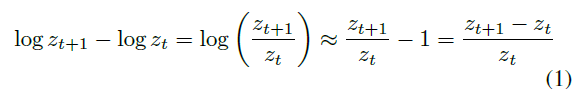
\includegraphics[width = \columnwidth]{images/formula-6.PNG}
\end{figure}
\end{comment}

\vspace{-0.25in}
\begin{figure}[htbp]
    \centering
    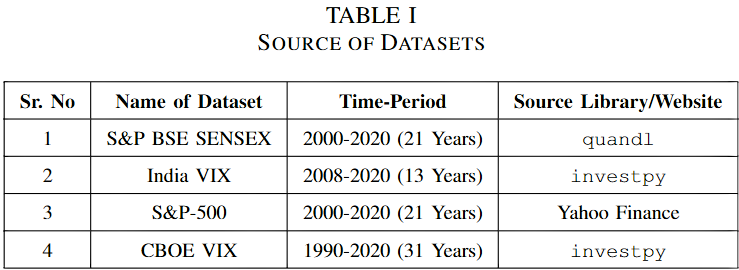
\includegraphics[width = \columnwidth]{images/source-of-datasets.PNG}
\end{figure}

Jarque Bera test is a goodness of fit statistical test that determines whether the numerical data skewness and kurtosis match a normal distribution \cite{b18} with the null hypothesis ($H_{0}$) and alternative hypothesis ($H_{A}$) defined as: \newline
$H_{0}: $ The given sequence is normally distributed. \newline
$H_{A}: $ The given sequence has another distribution.

A process is defined as a random walk if every value recorded is the result of a random event, and many financial time series data are modeled as random walk processes.
The Random Walk Process is governed by equations \eqref{eq: 2} - \eqref{eq: 4} as follows:

\begin{align}
    P_{t} = P_{t - 1} + \epsilon_{t} \label{eq: 2} \\
    P_{t} = d + P_{t - 1} + \epsilon_{t} \label{eq: 3} \\
    P_{t} = P_{0} + dt + \sum_{t = 1}^{n} \epsilon_{t} 
    \label{eq: 4}
\end{align}

\begin{comment}
\begin{figure}[htbp]
    \centering
    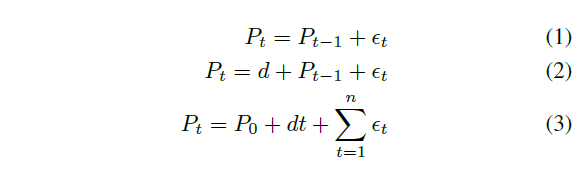
\includegraphics[width = \columnwidth]{images/formula-7.PNG}
\end{figure}
\end{comment}

\noindent where $P_{t} = $ Value of underlying series at time instant $t$. \\
$P_{t - 1} = $  Value of underlying series at time instant $t - 1$. \\
$d = $ Drift (which is just a trend like property for a random walk process, i.e.\\ $d > 0 \implies$ upward trend and $d < 0 \implies$ downward trend).\\
$\epsilon_{t} = $ white noise or Gaussian white noise.

\subsection{S\&P BSE SENSEX Index Exploratory Data Analysis (EDA)}
This section contains the results of an exploratory data analysis (EDA) done on S\&P BSE SENSEX index data.

\setcounter{table}{1}
\begin{table}[htbp]
    \caption{S\&P BSE SENSEX Daily Close and Daily Returns Descriptive Statistics}
	\resizebox{\columnwidth}{!}{%
	\begin{tabular}{| c | c | c | c |}
	\hline
	\textbf{Sr. No} & \textbf{Statistics} & \textbf{Daily Close} & \textbf{Daily Returns} \\
	\hline
		1              & Mean           & $17930.2$        & $0.0525427$ \\
	\hline
		2              & Median         & $17222.6$        & $0.0952336$ \\
	\hline
		3              & Min            & $2600.12$        & $-13.1526$ \\
	\hline
		4              & Max            & $47751.3$        & $17.3393$ \\
	\hline
		5              & Std. Dev       & $11379.9$        & $1.4641$ \\
	\hline
		6              & Skewness       & $0.401981$       & $-0.13972$ \\
	\hline
		7              & Kurtosis       & $-0.875044$      & $9.65161$ \\
	\hline
	\end{tabular}
	}
	\label{tab: s_and_p_bse_sensex_descriptive_stats}
\end{table}

\begin{table}[htbp]
    \centering
    \caption{S\&P BSE SENSEX Jarque Bera Test Statistics Results}
    \resizebox{0.80\columnwidth}{!}{%
    \begin{tabular}{|c|c|c|}
        \hline
         \textbf{Statistics} & \textbf{Daily Close} & \textbf{Daily Returns} \\
         \hline
         test-statistic & $307.514$ & $20257.592$ \\
         \hline
         p-value & $0.0$ & $0.0$ \\
         \hline
    \end{tabular}
    }
    \label{tab: s_and_p_bse_sensex_jarque_bera}
\end{table}

\begin{figure}[htbp]
    \centering
	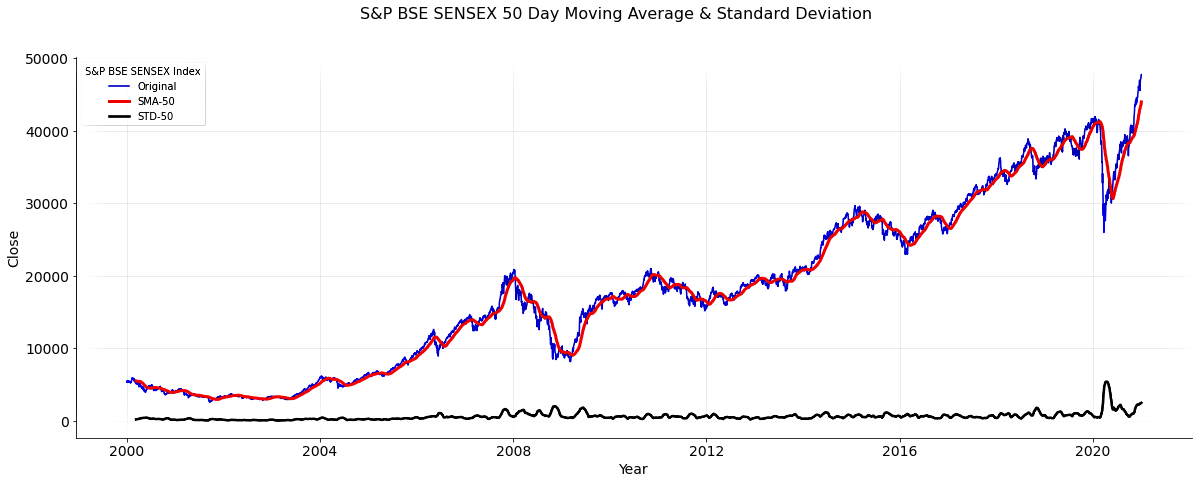
\includegraphics[scale = 1.5, width = 0.50 \textwidth]{images/SENSEX-Line-Plot.png}
	\vspace{-0.3in}
	\caption{S\&P BSE SENSEX Index Daily Close Values (2000-2020)}
	\label{fig: s_and_p_bse_sensex_line_plot}
	\vspace{0.1in}
	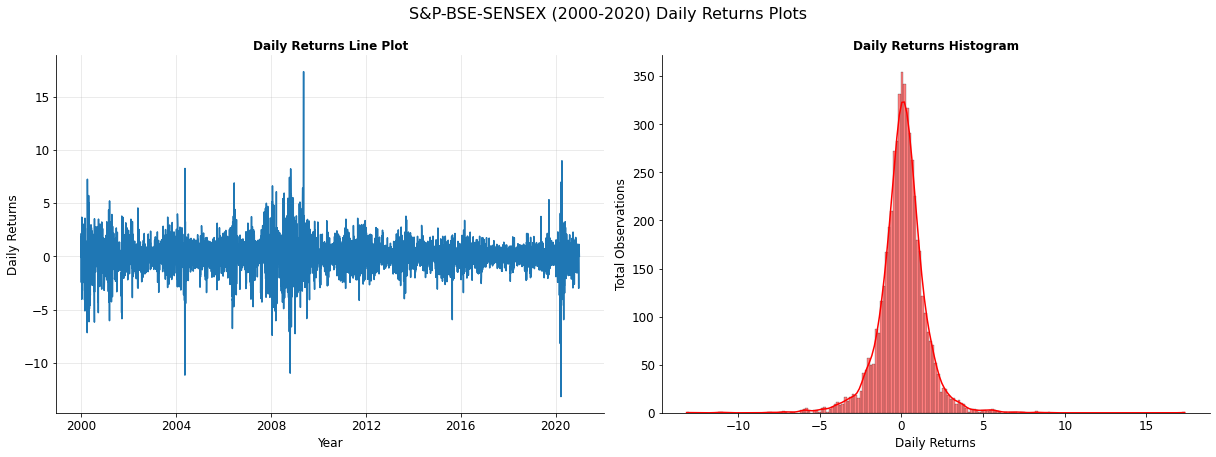
\includegraphics[scale = 1.5, width = 0.50 \textwidth]{images/SENSEX 2000-2020 Change Plot.png}
	\vspace{-0.3in}
	\caption{S\&P BSE SENSEX Daily Returns Plot (2000-2020)}
	\label{fig: s_and_p_bse_sensex_percentage_change_plot_1}
	\vspace{0.1in}
	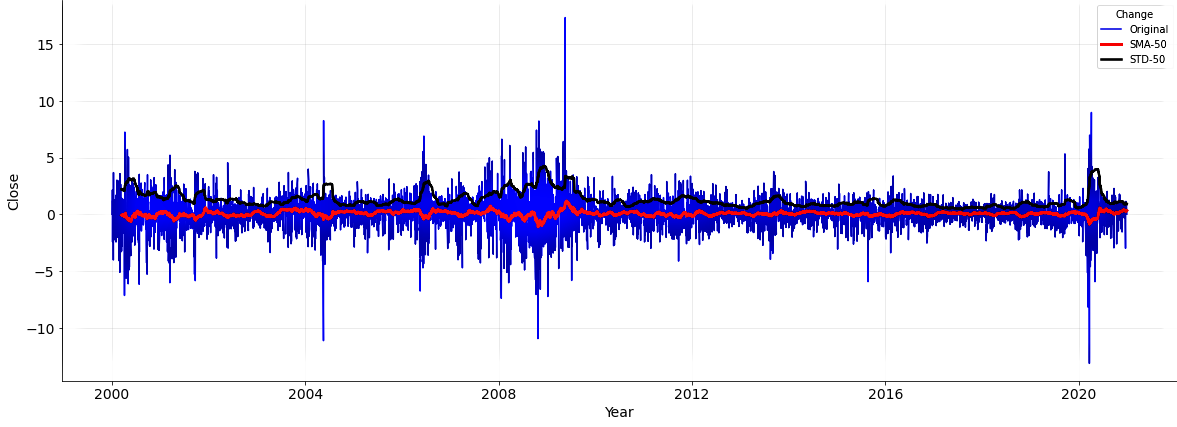
\includegraphics[scale = 1.5, width = 0.50 \textwidth]{images/BSE SENSEX White Noise Part.png}
	\vspace{-0.3in}
	\caption{S\&P BSE SENSEX Daily Returns Plot with 50-Day Moving Average and Standard Deviation}
	\label{fig: s_and_p_bse_sensex_percentage_change_plot_2}
\end{figure}

\subsection{S\&P-500 Index Exploratory Data Analysis}
This section contains the results of an exploratory data analysis (EDA) done on S\&P-500 index data.

\begin{table}[htbp]
    \caption{S\&P-500 Daily Close and Daily Returns Descriptive Statistics}
	\resizebox{\columnwidth}{!}{%
	\begin{tabular}{| c | c | c | c |}
	\hline		
	\textbf{Sr. No} & \textbf{Statistics}   & \textbf{Daily Close} & \textbf{Daily Returns} \\
	\hline
		1              & Mean             & $1653.27$        & $0.025695$           \\
	\hline
		2              & Median           & $1386.95$        & $0.0593618$          \\
	\hline
		3              & Min              & $676.53$         & $-11.9841$           \\
	\hline
		4              & Max              & $3735.36$        & $11.58$              \\
	\hline
		5              & Std. Dev         & $673.836$        & $1.25313$            \\
	\hline
		6              & Skewness         & $1.03217$        & $-0.1538$            \\
	\hline
		7              & Kurtosis         & $0.0629593$      & $10.736$             \\
	\hline
	\end{tabular}
	}
	\label{tab: s_and_p_500_statiscal_analysis}
\end{table}

\begin{table}[htbp]
    \centering
    \caption{S\&P-500 Jarque Bera Test Statistics Results}
    \resizebox{0.80\columnwidth}{!}{%
    \begin{tabular}{|c|c|c|}
    \hline
         \textbf{Statistics} & \textbf{Daily Close} & \textbf{Daily Returns} \\
    \hline
         test-statistic &  $938.37$ & $25339.39$ \\
    \hline
         p-value & $0.0$ & $0.0$ \\
    \hline
    \end{tabular}
    \label{tab:s_and_p_500_jarque_bera_stats}
    }
\end{table}

\begin{figure}[htbp]
	\centering
	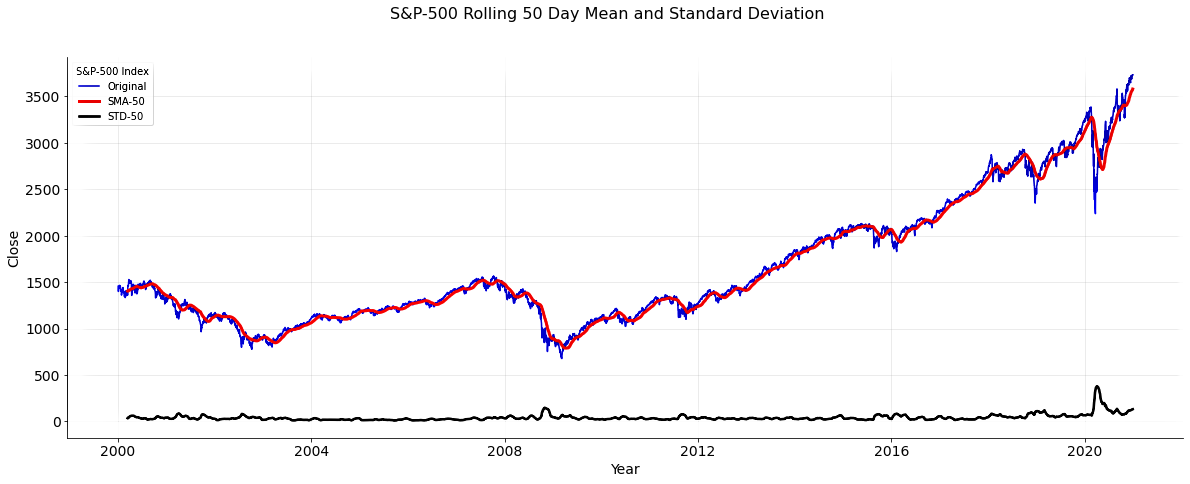
\includegraphics[scale = 1.5, width = 0.52 \textwidth]{images/S&P-500 Line Plot.png}
	\vspace{-0.3in}
	\caption{S\&P-500 Index Daily Close Values (2000-2020)}
	\label{fig: s_and_p_500_index_line_plot}
	
	\vspace{0.1in}
	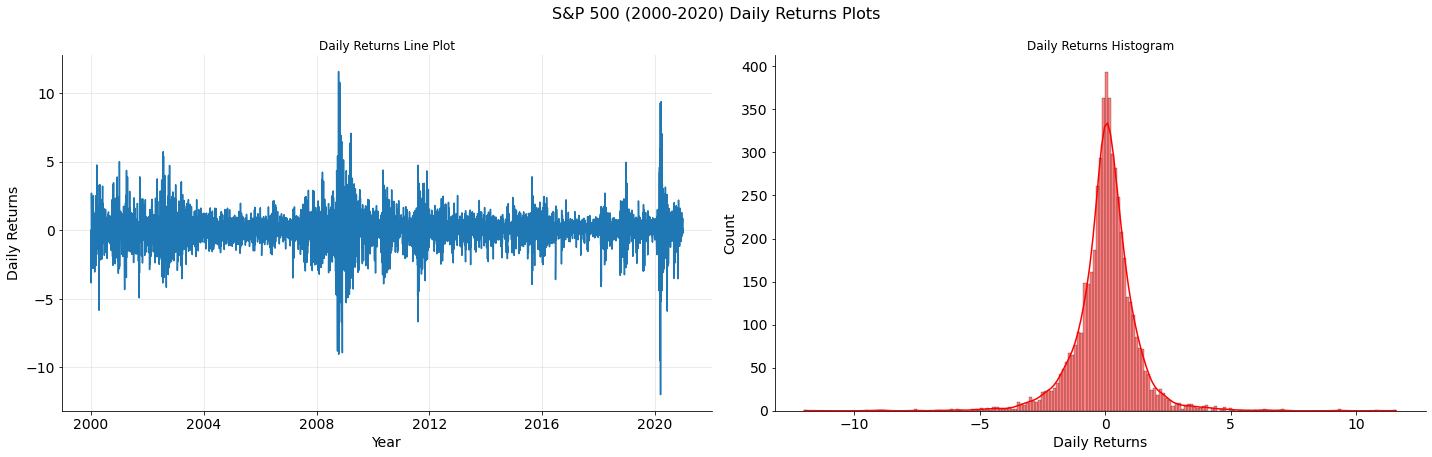
\includegraphics[scale = 1.5, width = 0.54 \textwidth]{images/S&P-500 Change Plot.png}
	\vspace{-0.3in}
	\caption{S\&P-500 Daily Returns Plots (2000-2020)}
	\label{fig: s_and_p_500_percentage_change_plot_1}
	
	\vspace{0.1in}
	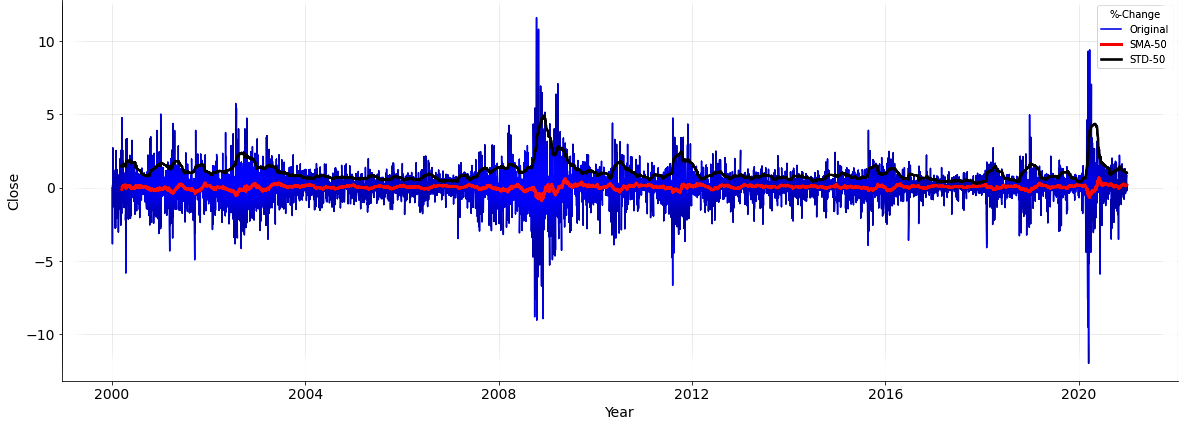
\includegraphics[scale = 1.5, width = 0.52 \textwidth]{images/S&P-500 White Noise Part.png}
	\vspace{-0.3in}
	\caption{S\&P-500 Daily Returns Plot with 50-Day Moving Average and Standard Deviation}
	\label{fig: s_and_p_500_percentage_change_plot_2}
\end{figure}

\subsection{Conclusions from Exploratory Data Analysis (EDA)}
The conclusions obtained after performing exploratory data analysis on India and USA benchmark index data are as follows:

\begin{itemize}
    \item Table \ref{tab: s_and_p_bse_sensex_descriptive_stats} and \ref{tab: s_and_p_500_statiscal_analysis} shows the basic statistical values such as mean, standard deviation, max, min, skewness and kurtosis computed for S\&P BSE SENSEX and S\&P-500 indexes.
    
    \item From Figs. \ref{fig: s_and_p_bse_sensex_line_plot} and \ref{fig: s_and_p_500_index_line_plot} it is observed that there is a trend component present in both the indexes time series data and statistical properties like mean ($\mu$), standard deviation ($\sigma$) and variance ($s$) are dependent on time.
    
    \item After performing Jarque Bera statistical test for daily close and daily returns of India and USA benchmark index, the p-value was found to be $< 0.05$ and test statistic is farther away from zero (refer Table \ref{tab: s_and_p_bse_sensex_jarque_bera} and \ref{tab:s_and_p_500_jarque_bera_stats}) implies that the observations are not normally distributed.
    
    \item From Figs. \ref{fig: s_and_p_bse_sensex_percentage_change_plot_1} and \ref{fig: s_and_p_500_percentage_change_plot_1}, the daily returns value plot resembles with white noise process as first difference shown in Figs. \ref{fig: s_and_p_bse_sensex_percentage_change_plot_2} and \ref{fig: s_and_p_500_percentage_change_plot_2} has mean ($\mu$) $\approx 0$ and std. dev ($\sigma$) is constant implies that the underlying India and USA benchmark indexes are random walk processes.
\end{itemize}

\subsection{Volatility Indexes (VIX)}
VIX Indexes allow measuring quantitatively in real-time, near-term volatility expectations of the market from the perspective of the future and options market. Fig. \ref{fig:india_vix_index} shows the India VIX index \footnote{India VIX helps to measure the near-term volatility of the Indian equity market was launched in 2007 \& computed by NSE where the computation is based completely on the order book of NIFTY Futures \& Options (F\&O).} and Fig. \ref{fig:cboe_vix_index} shows the CBOE VIX index \footnote{The CBOE volatility index forecasts how volatile the S\&P-500 index will be over the following 30 trading sessions based on the pricing of put and call options on the index.} 
For the computation of India VIX values, the most appropriate bid-ask excerpt of near ($\sigma_{V_{1}}$) and next-month ($\sigma_{V_{2}}$) NIFTY options contracts traded on the F\&O segment of NSE are considered \cite{b4}. The equations from \eqref{eq: 5} - \eqref{eq: 7} are used for the computation of India VIX:

\begin{align}
    \sigma^{2}_{V} = \frac{2}{T_{v}} \sum_{i}\frac{\Delta  K_{v_{i}}}{K_{v_{i^{2}}}}e^{{R_{v}T_{v}}}Q(K_{v_{i}}) - \frac{1}{T_{v}}\Big[\frac{F_{v}}{k_{0}} - 1\Big]^2 \label{eq: 5}
\end{align}

\begin{comment}
\begin{figure}[htbp]
    \centering
    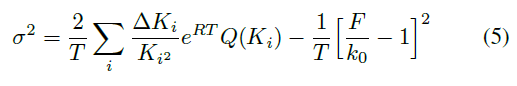
\includegraphics[width = 0.90\columnwidth]{images/formula-1.PNG}
\end{figure}
\vspace{-0.2in}
\end{comment}

\noindent where $T_{v} =$ Time to expiration, $K_{v_{i}} = $ Strike price of $i^{th}$ out of money option, a call if $K_{v_{i}} > F_{v}$ and a put if $K_{v_{i}} < F_{v}$

\noindent $\Delta K_{v_{i}} =$ computed using equation \eqref{eq: 6} denotes the interval between strike prices on either side of $K_{v_{i}}$.
    
\begin{align}
    \Delta K_{v_{i}} = \frac{K_{v_{i + 1}} - K_{v_{i - 1}}}{2} \label{eq: 6}
\end{align}
    
\begin{comment}
\vspace{-0.2in}
\begin{figure}[htbp]
    \centering
    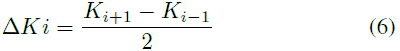
\includegraphics[width = 0.70\columnwidth]{images/formula-2.PNG}
\end{figure}
\vspace{-0.15in}
\end{comment}

\noindent $R_{v} =$ Risk-free interest rate of expiration.
$Q(K_{v_{i}}) =$ A bid-ask price at the middle of each option contract with strike $K_{i}$. \newline
$F_{v} =$ The last price of the NIFTY futures contract with a corresponding expiration is used to calculate the forward index. $k_{0} =$ First strike below the $F_{v}$. \newline
India VIX values are determined by individually computing the near month ($\sigma_{V_{1}}$) and next month ($\sigma_{V_{2}}$) VIX values with time to expiration of $T_{1}$ and $T_{2}$ respectively and then ${\sigma^{2}_{V}}$ value is derived by interpolating $\sigma_{V_{1}}$ and $\sigma_{V_{2}}$ according to equation \eqref{eq: 7}:

\begin{align}
   \sigma_{V}^{2} = \Big\{T_{1}{\sigma_{V_{1}}}^{2}\Big[\frac{N_{T_{2}} - N_{30}}{N_{T_{2}} - N_{T_{1}}}\Big] + T_{2}{\sigma_{V_{2}}}^{2}\Big[\frac{N_{30} - N_{T_{1}}}{N_{T_{2}} - N_{T_{1}}}\Big]\Big\} \times \frac{N_{365}}{N_{30}} \label{eq: 7}
\end{align}

\begin{comment}
\vspace{-0.2in}
\begin{figure}[htbp]
    \centering
    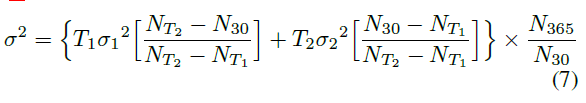
\includegraphics[width = \columnwidth]{images/formula-3.PNG}
\end{figure}
\vspace{-0.18in}
\end{comment}

\noindent where: $N_{T_{1}} =$ The total minutes until the near month options expire $= 12960$ and $N_{T_{2}} =$ The total minutes until the next month options expire $= 53280$. \newline

$N_{30} =$ Total minutes in $30$ days $= 43200$ and $N_{365} =$ total minutes in $365$ days $= 525600$. \newline

The India VIX ($\sigma_{V}^{2}$) measures the predicted market volatility over the next 30 trading sessions, with higher values reflecting greater volatility and vice versa.

% For more detailed information on how the values of India VIX are computed, please refer the white paper published by National Stock Exchange (NSE) \cite{b4} on how the computation is done with examples.

% The index is also refered as "investor fear index", the CBOE VIX is a measure of the implied volatility of the SPX, and is observed to be correlated with the 30-day realized volatility of the SPX. Changes in the CBOE VIX are observed to be negatively correlated with changes in the SPX.

% The CBOE Volatility Index (VIX) quantitatively measures the market's expectations for the relative strength of near-term price changes of the S\&P 500 index (SPX) because it's derived from the prices of SPX index options with near-term expiration dates, it generates a $30$-day forward projection of volatility.

\begin{figure}[htbp]
	\centering
	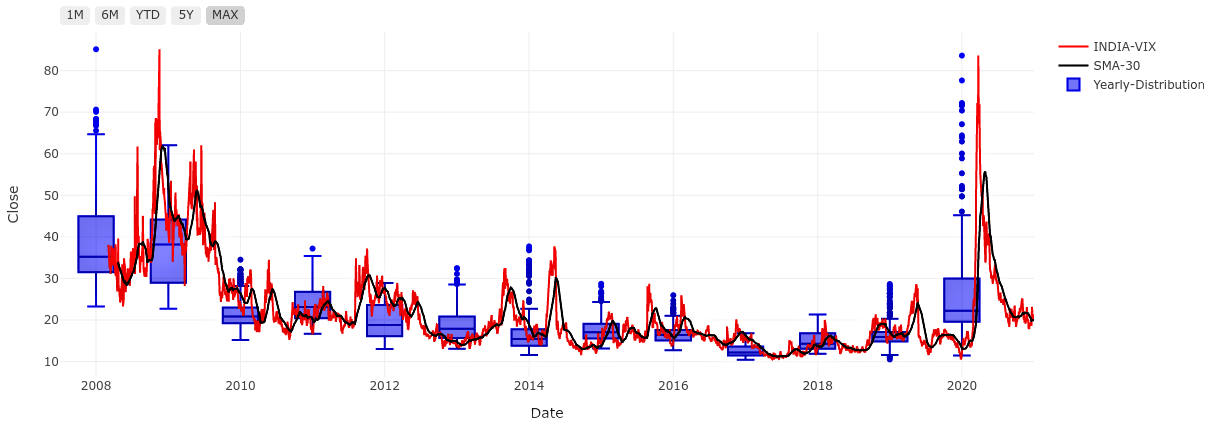
\includegraphics[scale = 1.5, width = 0.50 \textwidth]{images/INDIA-VIX (2008-2020).png}
	\vspace{-0.3in}
	\caption{India VIX Index (2008-2020) Plot}
	\label{fig:india_vix_index}
	
	\vspace{0.1in}
	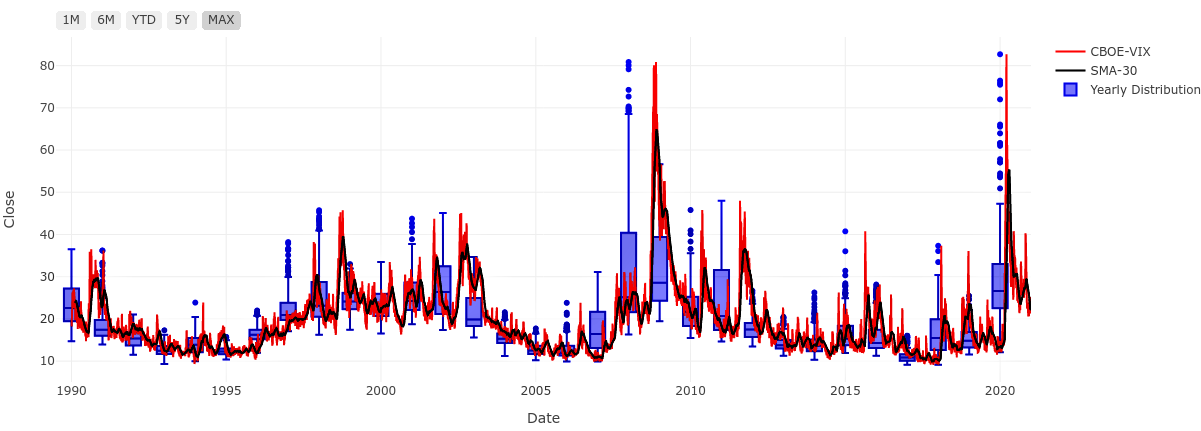
\includegraphics[scale = 1.5, width = 0.50 \textwidth]{images/CBOE-VIX.png}
	\vspace{-0.3in}
	\caption{Chicago Board of Exchange (CBOE) VIX Index (1990-2020) Plot}
	\label{fig:cboe_vix_index}
\end{figure}

S\&P BSE SENSEX and S\&P-500 indexes daily close value ACF plot (Fig. 9 and 11) are unity ($\approx 1$) for short-term lags and decays to $0$ at $\approx 1900^{th}$ lag. One of the properties of the random walk process states if the number of observations is high enough then the autocorrelation coefficient ($\rho_{k}$) is almost unity because the autocorrelation coefficient ($\rho_{k}$) of random walk process is dependent on time ($t$) as derived from equations \eqref{eq: 8} to \eqref{eq: 10} where $Cov(a_{t}, a_{t+k})$ represents the covariance and $Var(a_{t})$, $Var({a_{t + k}})$ represents the variance:

\begin{align}
\rho_{k}(t) = \frac{Cov(a_{t}, a_{t+k})}{\sqrt{Var(a_{t}) \times Var(a_{t + k})}} \label{eq: 8}& \\ = \frac{t\sigma^{2}}{\sqrt{t\sigma^{2}\times(k + t)\times \sigma^{2}}} \label{eq: 9}
\end{align}

\begin{comment}
\vspace{-0.2in}
\begin{figure}[htbp]
    \centering
    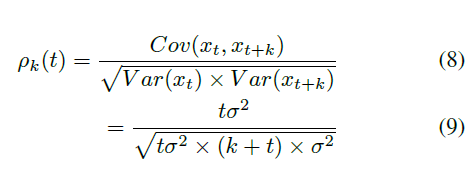
\includegraphics[width = 0.8 \columnwidth]{images/formula-4.PNG}
\end{figure}
\vspace{-0.15in}
\end{comment}

Rearranging the terms will give the following equation for autocorrelation coefficient ($\rho_{k}$) for a random walk process:

\begin{align}
    \rho_{k} = \frac{1}{\sqrt{1 + (k / t)}} \label{eq: 10}
\end{align}

\begin{comment}
\begin{figure}[htbp]
    \centering
    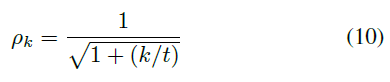
\includegraphics[width = 0.70 \columnwidth]{images/formula-5.PNG}
\end{figure}
\end{comment}

From equation (10), autocorrelation coefficient ($\rho_{k}$) is inversely related to time ($t$) hence autocorrelation coefficient ($\rho_{k}$) value was unity $\approx 1$ for shorter time lags in Figs. \ref{fig: s_and_p_bse_sensex_acf_and_pcf_plots} and \ref{fig: s_and_p_500_acf_and_pacf_plots}.
\subsection{ACF and PACF Plots}
% The Figs. \ref{fig: s_and_p_bse_sensex_acf_and_pcf_plots}, \ref{fig: s_and_p_bse_sensex_percentage_change_acf_and_pacf_plots}, \ref{fig: s_and_p_500_acf_and_pacf_plots}, and \ref{fig: s_and_p_500_percentage_change_acf_and_pacf_plots} shows the auto-correlation function (ACF) and partial auto-correlation functions (PACF) plots for S\&P BSE SENSEX and S\&P-500 indexes to understand the relationships/dependency between the value the given financial time series data i.e. S\&P BSE SENSEX and S\&P-500 indexes has taken at time $t$ and time $t - 1$.

For India and USA benchmark indexes, the daily returns ACF plot in Figs. \ref{fig: s_and_p_bse_sensex_percentage_change_acf_and_pacf_plots} and \ref{fig: s_and_p_500_percentage_change_acf_and_pacf_plots} doesn't show any statistically significant correlation at lags $k$ and $95\%$ of the spikes in both the ACF plots are in the range of $\pm 2/\sqrt{T}$ where $T$ represents the number of observations which implies the underlying daily returns sequence is a white noise process.

\onecolumn
\begin{figure}[htbp]
	\centering
	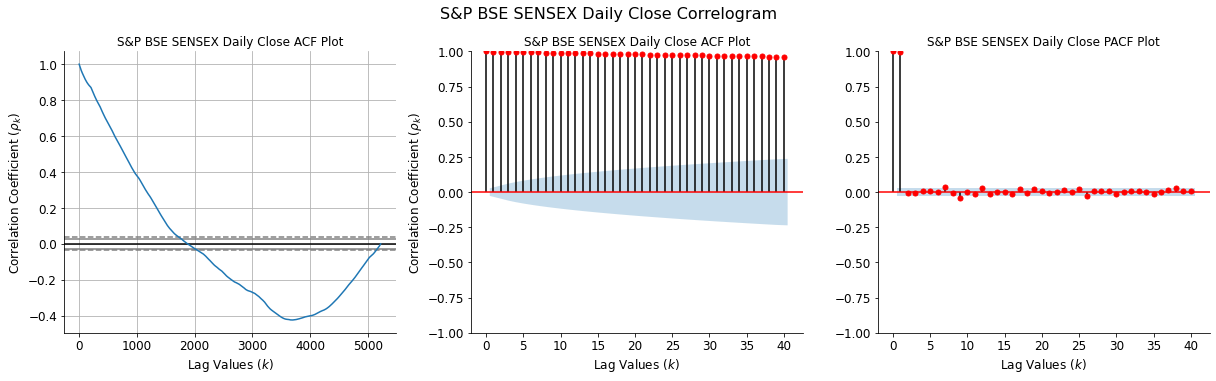
\includegraphics[scale = 1.5, width = \textwidth]{images/SENSEX ACF and PACF Plot.png}
	\vspace{-0.3in}
	\caption{S\&P BSE SENSEX Daily Close Value (2000-2020) ACF and PACF Plots}
	\label{fig: s_and_p_bse_sensex_acf_and_pcf_plots}
	
	\vspace{0.1in}
	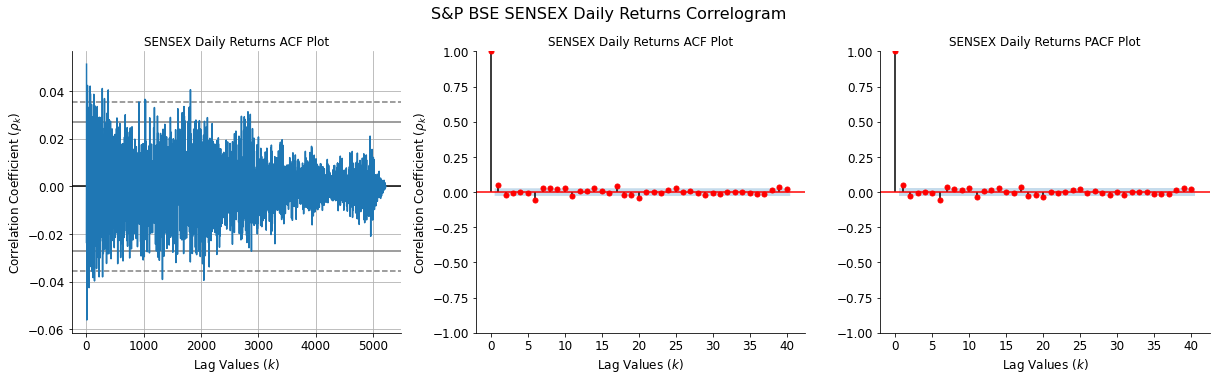
\includegraphics[scale = 1.5, width = \textwidth]{images/SENSEX Change ACF, PACF Plots.png}
	\vspace{-0.3in}
	\caption{S\&P BSE SENSEX Daily Returns Value (2000-2020) ACF and PACF Plots}
	\label{fig: s_and_p_bse_sensex_percentage_change_acf_and_pacf_plots}
	
	\vspace{0.1in}
	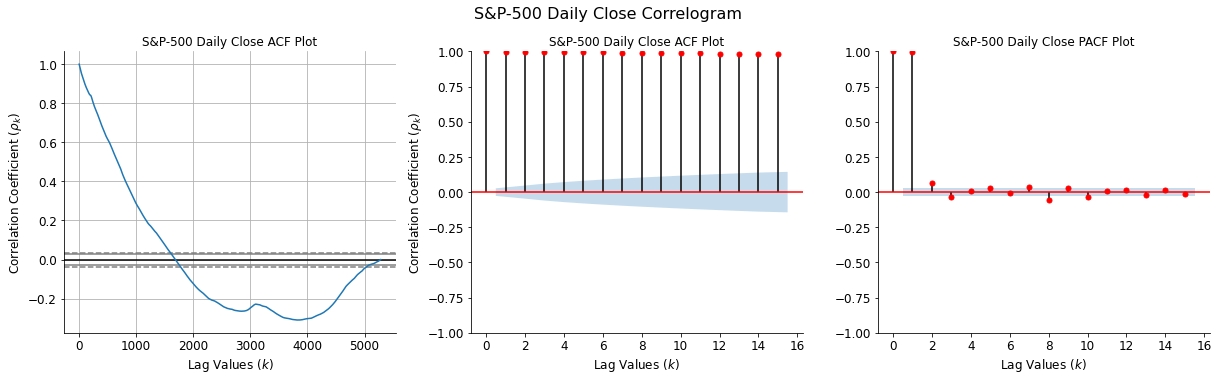
\includegraphics[scale = 1.5, width = \textwidth]{images/S&P-500 ACF, PACF Plots.png}
	\vspace{-0.3in}
	\caption{S\&P-500 Daily Close Value (2000-2020) ACF and PACF Plots}
	\label{fig: s_and_p_500_acf_and_pacf_plots}
	
	\vspace{0.1in}
	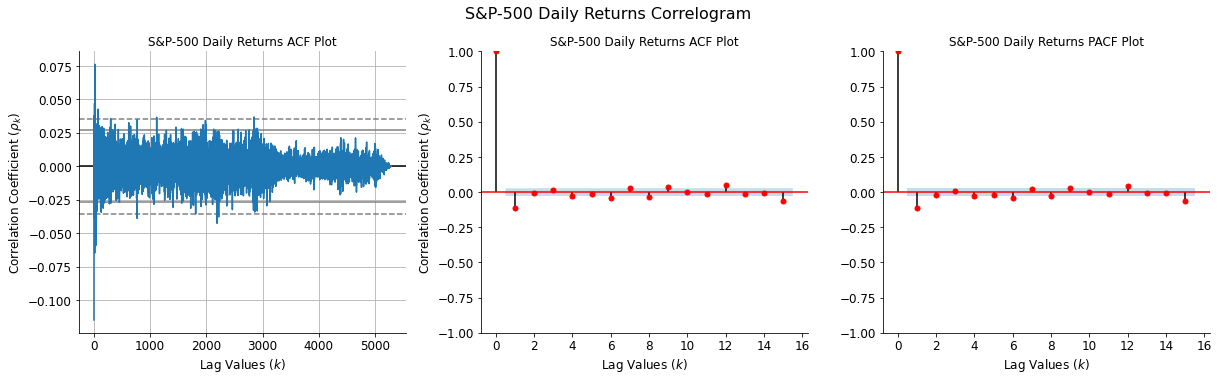
\includegraphics[scale = 1.5, width = \textwidth]{images/S&P-500 Change ACF PACF Plot.png}
	\vspace{-0.3in}
	\caption{S\&P-500 Daily Returns Value (2000-2020) ACF and PACF Plots}
	\label{fig: s_and_p_500_percentage_change_acf_and_pacf_plots}
\end{figure}

\twocolumn

The interesting insights from Figs. \ref{fig:india_vix_index} and \ref{fig:cboe_vix_index} are in the FY-2009 and FY-2021, the volatility observed in the both India \& USA equity markets were very high due to the following events:
\begin{itemize}
    \item In FY-2009 global financial crisis happened as a result of the crash of the mortgage market in the USA due to bad loans and the fall of AAA-rated Credit Debt Obligations (CDOs) and 
    \item In FY-2021 due to COVID-19, a sequence of events happened as a result of the great lockdown which led to the panic selling of securities as seen in the markets globally caused by the fear of recession in investors.
\end{itemize}

\section{Statistical Tests for Stationarity} \label{statistical_tests}
\subsection{Augmented Dickey-Fuller (ADF) Statistical Test}
The Augmented Dickey-Fuller (ADF) test is one of the several unit root tests to assess the stationarity of TS data where null hypothesis ($H_{0})$ and alternative hypothesis ($H_{A})$ as described below:

$H_{0}$: Given time series data is non-stationarity $\implies$ Time series data has time-dependent statistical properties i.e., mean, variance, auto-correlation, etc. present in it.

$H_{A}:$ Given time series data is stationary, $\implies$ time series data doesn't have any time-dependent statistical properties present in it. \newline
If the p-value obtained is $\le 0.05 \implies$ Reject, the $H_{0}$ otherwise $\implies$ Failed to Reject $H_{0}.$ \newline
Table \ref{tab: s_and_p_bse_sensex_adf_test_results} and \ref{tab: s_and_p_500_adf_test_results} shows the results of Augmented Dickey Fuller Statistical Test performed on both the indexes.

\begin{table}[htbp]
    \centering
	\caption{S\&P BSE SENSEX Augmented Dickey Fuller Test Results}
	\resizebox{\columnwidth}{!}{%
	\renewcommand{\arraystretch}{1.5}
	\begin{tabular}{|c|c|c|c|c|}
		\hline
		\textbf{Sr. No} & \textbf{Data} & \textbf{t-statistic} & \textbf{p-value} & \textbf{Verdict}        \\
		\hline
		1 & Daily Close Values  & $0.688133$ & $0.989598$ & Failed to Reject $H_{0}$. \\
		\hline
		2 & Daily Returns Values & $-16.081$  & $5.390 \times 10^{-29}$ & Reject $H_{0}$.\\
		\hline
	\end{tabular}
	}
	\label{tab: s_and_p_bse_sensex_adf_test_results}
\end{table}

From Table \ref{tab: s_and_p_bse_sensex_adf_test_results} the p-value obtained for S\&P BSE SENSEX daily close values is $0.989598 > 0.05 \;(\alpha) \implies$ Failed to Reject $H_{0} \implies$ S\&P BSE SENSEX daily close values is \textbf{non-stationary} and p-value obtained for S\&P BSE SENSEX daily returns values is $5.389647 \times 10^{-27} << 0.05 \;(\alpha) \implies$ Reject the $H_{0} \implies$ S\&P BSE SENSEX daily returns values is \textbf{stationary}.

\begin{table}[htbp]
	\caption{S\&P-500 Augmented Dickey Fuller Test Results.}
	\resizebox{\columnwidth}{!}{%
	\renewcommand{\arraystretch}{1.5}
	\begin{tabular}{|c|c|c|c|c|}
		\hline
		\textbf{Sr. No} & \textbf{Data} & \textbf{t-statistic} & \textbf{p-value} & \textbf{Verdict}        \\
		\hline
		1 & Daily Close Values & $1.631761$ & $0.99795$ & Failed to Reject $H_{0}$. \\
		\hline
		2 & Daily Returns Values & $-13.742$ & $1.095 \times 10^{-25}$ & Reject $H_{0}$.    \\
		\hline
	\end{tabular}
	}
	\label{tab: s_and_p_500_adf_test_results}
\end{table}

From Table \ref{tab: s_and_p_500_adf_test_results} the p-value obtained for S\&P-500 daily close values is $0.99795 > 0.05 \;(\alpha) \implies$ Failed to Reject $H_{0} \implies$ S\&P-500 daily close values is \textbf{non-stationary} and p-value obtained for S\&P-500 daily returns values is $1.094051 \times 10^{-25} << 0.05 \;(\alpha) \implies $ Reject the $H_{0} \implies$ S\&P-500 daily returns values is \textbf{stationary}.

\section{Estimating Parameters of Models} \label{estimating_parameters_of_models}
A general category of TS models called ARIMA becomes necessary, which is also known as Box-Jenkins models since they use a structured approach to check, identify, fit, and leverage the ARIMA models that George Box and Gwilym Jenkins first proposed in 1976 \cite{b6}.
ARIMA models are an extension of ARMA models when dealing with non-stationary TS data, i.e., when the statistical attributes (mean, variance, standard deviation) of TS data changes with time. The ARIMA model mathematically represented as $ARIMA(p, d, q)$, where $p, q \;\text{and}\; d$ are order of AR process, order of MA process, and order of differencing.
This study uses a seasonal ARIMA model (SARIMA), but there is a requirement for exposing the SARIMA model to a set of exogenous features on which the model will not auto-regressed but will influence its forecast at time $t$. As a result, the model used is SARIMAX, where X represents the set of exogenous features \cite{b17}.

For $n$ exogenous given variables defined at time step $t$, represented by $x_{t}$ for $i \leq n$ with coefficient $\beta_{i}$ is given by equation \eqref{eq: 11} for $SARIMAX(p,d,q)(P,D,Q,s)$ model \cite{b17} respectively.

\begin{align}
    \Theta(L)^{p} \theta(L^{s})^{P} \Delta^{d} \Delta_{s}^{D} y_{t} = \Phi(L)^{q} \phi(L^{s})^{Q} \Delta^{d} \Delta_{s}^{D} \epsilon_{t} + \sum_{i=1}^{n} \beta_{i} x^{i}_{t}
    \label{eq: 11}
\end{align}

The exogenous variables (X) used for the training of the corresponding SARIMAX model are lag based features because they are useful in providing past information about assorted trends present in the underlying indexes time series data and are extracted from the dataset itself i.e., standard deviation and moving averages for $3, 7, 30, 50, 100$ days of the indexes high and low values for each trading day. Therefore, to forecast the future values of indexes, these exogenous variables also have to be added to the trained time series model during forecasting.

For Prophet\cite{b7} library-based predictions, there is no need to estimate parameters because the library has abstracted that process and the same set of exogenous features was used as in the SARIMAX during the training and forecasting of Prophet models.
Coefficients of SARIMAX equations were determined through step wise search algorithm used by \mintinline{python}{pmdarima.arima.auto_arima()} method defined in the \mintinline{python}{pmdarima} library when performing hyperparameter optimization.

\subsection{S\&P BSE SENSEX Index}
Estimated hyperparameters of SARIMAX are: SARIMAX $(2, 0, 1)(2, 0, 0, 7)$ with an AIC $\approx 64126.053$ for India benchmark index and SARIMAX $(5, 1, 1)(2, 0, 1, 7)$ with an AIC $\approx 35713.686$ for the USA benchmark index.

\section{Validation For Actual and Forecasted Values} \label{validation_for_actual_and_forecasted_values}

\begin{figure*}[ht]
	\centering
	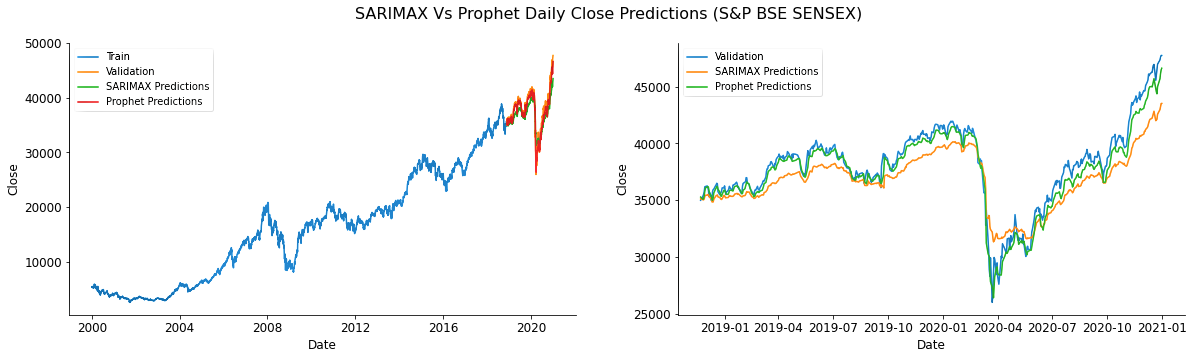
\includegraphics[scale = 1.5, width = \textwidth]{images/SARIMAX-Prophet-SENSEX-Predictions.png}
	\vspace{-0.3in}
	\caption{SARIMAX and Prophet Model Daily Close Value Predictions On Validation Dataset for S\&P BSE SENSEX}
	\label{fig:sarimax_prophet_results_sensex_index}
\end{figure*}

\begin{figure*}[ht]
	\centering
	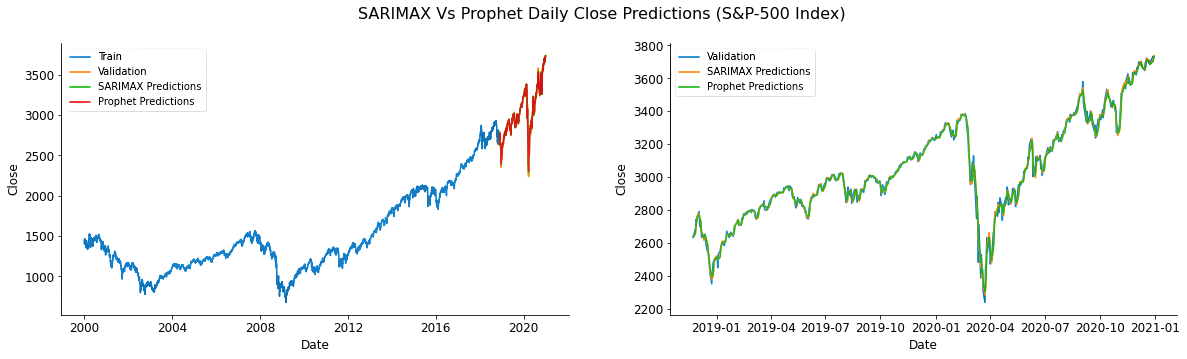
\includegraphics[scale = 1.5, width = \textwidth]{images/SARIMAX-Prophet-S&P-500-Predictions.png}
	\vspace{-0.3in}
	\caption{SARIMAX and Prophet Model Daily Close Value Predictions On Validation Dataset for S\&P-500}
	\label{fig: sarimax_prophet_results_for_s_and_p_500_index}
\end{figure*}

The given financial TS data for training SARIMAX and Prophet is divided in the ratio of $90:10$ by retaining the temporal characteristics of the data implies $90\%$ of the data consumed for training and the remainder $10\%$ used as validation data to evaluate the model performance. After the training phase is over the models (SARIMAX and Prophet) are evaluated using various metrics such as Mean Absolute Error (MAE), Mean Square Error (MSE), Root Mean Square Error (RMSE), $R^{2}$ value, and Mean Absolute Percentage Error (MAPE) with more emphasis given to $R^{2}$ value and Mean Absolute Percentage Error (MAPE).

\subsection{S\&P BSE SENSEX Index}
The Fig. \ref{fig:sarimax_prophet_results_sensex_index} shows the performance of the models (SARIMAX and Prophet) on validation dataset of S\&P BSE SENSEX.

\begin{table}[htbp]
    \centering
    \caption{SARIMAX and Prophet Error Metric Values}
    \resizebox{0.90\columnwidth}{!}{%
    \begin{tabular}{|c|c|c|c|}
        \hline
        \textbf{Sr. No} & \textbf{Metrics} &  \textbf{SARIMAX} & \textbf{Prophet} \\
        \hline
        1 & MAE & 1553.14 & 611.33 \\
        \hline
        2 & MSE & $3.39 \times 10^{6}$ & $5.998 \times 10^{5}$ \\
        \hline
        3 & RMSE & 1839.91 & 774.44 \\
        \hline
        5 & $R^{2}$ value $[0, 1]$ & 0.7314 & 0.95 \\
        \hline
        6 & MAPE & $4.05 \%$ & $1.60\%$ \\
        \hline
    \end{tabular}
    }
    \label{tab:s_and_p_sensex_model_evaluation_metric_table}
\end{table}

\subsection{S\&P-500 Index}
The Fig. \ref{fig: sarimax_prophet_results_for_s_and_p_500_index} graphs shows the performance of the models (SARIMAX and Prophet) on validation dataset of S\&P-500.

\begin{table}[ht]
    \centering
    \caption{SARIMAX and Prophet Error Metric Values}
    \resizebox{0.90\columnwidth}{!}{%
    \begin{tabular}{|c|c|c|c|}
        \hline
        \textbf{Sr. No} & \textbf{Metrics} &  \textbf{SARIMAX} & \textbf{Prophet} \\
        \hline
        1 & MAE & 18.189 & 18.452 \\
        \hline
        2 & MSE & 755.416 & 770.787 \\
        \hline
        3 & RMSE & 27.485 & 27.764 \\
        \hline
        5 & $R^{2}$ value $[0, 1]$ & 0.991685 & 0.991516 \\
        \hline
        6 & MAPE & $0.62 \%$ & $0.63\%$ \\
        \hline
    \end{tabular}
    }
    \label{tab: s_and_p_500_model_evaluation_metric_table}
\end{table}

\section{Findings from the Study} \label{findings_from_study}
$R^{2}$ value known as coefficient of determinism helps in understanding how much variance the model is able to explain/capture out of the total variance present in the numerical sequence and higher the $R^{2}$ value the better the model fit. From Table \ref{tab:s_and_p_sensex_model_evaluation_metric_table} and \ref{tab: s_and_p_500_model_evaluation_metric_table}, SARIMAX $(2, 0, 0)(2, 0, 0, 7)$ for India benchmark index and SARIMAX $(5, 1, 1)(2, 0, 1, 7)$ for the USA benchmark index yielded reliable results with a $R^{2}$ values of $0.731307$ and $0.991685$ and mean average precision error (MAPE) of $4.05\%$ and $0.61\%$. Prophet has outperformed the corresponding SARIMAX models when forecasting the underlying India and USA benchmark indexes, with $R^{2}$ values of $0.952397$ and $0.991516$, respectively, and mean average precision errors (MAPE) of $1.06\%$ and $0.62\%$. However, from Figs. \ref{fig:sarimax_prophet_results_sensex_index} and \ref{fig: sarimax_prophet_results_for_s_and_p_500_index} actual and predicted daily close values differ significantly which is captured by mean absolute error (MAE) evaluation metric in table \ref{tab:s_and_p_sensex_model_evaluation_metric_table} and \ref{tab: s_and_p_500_model_evaluation_metric_table}, but the models (SARIMAX and Prophet) can capture the assorted trends and volatility present in both the indexes historical data during the training phase with Prophet being better and more reliable than SARIMAX when tested on validation dataset.

From the application perspective, these models can be used as an approximate technical indicator of what daily close values the indexes would take or can be used to determine the approximate trends in market indexes in short term to manage/optimize the portfolios to maximize the profits.

\section{Conclusions} \label{conclusions}
Several studies in the research community have been undertaken on the forecasting of stock/equity market returns utilizing classic ARIMA and other sophisticated models, particularly for developed economies such as the United States and Europe. However, less focus is given to emerging/developing and less developed economies and a comparison of developed economies with developing ones. Moreover, indexes of any stock market gauge the sentiment of the market tells about the growth of the underlying economy and how the local dynamics affect/drive the value of the market indexes \cite{b5} which helps to make a comparison about which market is going to do well in the future, emerging market like Indian stock market or developed market like the United States stock market based on the fluctuations, trends forecasted by the developed models.
This paper fills the gap by forecasting daily close values of S\&P BSE SENSEX (Emerging Market Index) and S\&P-500 (Developed Market Index) using SARIMAX and Prophet time series model with Prophet-based model in both the index cases turns out to be more accurate and reliable than its SARIMAX counterpart as per section \ref{findings_from_study}.

Incorporating more exogenous variables into the dataset, such as price to earnings ratio (P/E Ratio), price to book value ratio (P/B Ratio), shared traded, consumer price index (CPI), wholesale price index (WPI), gross domestic product (GDP), $\beta$ value as a risk measurement \cite{b3} etc., can aid in the development of more robust and reliable forecasting models.

The markets not only tell us the sentiment of the investor in the short-term as a reflection of the information available but also gives us an idea about what are the variables that play a major role such as budget announcements, stimulus plans, government policies, and political events, foreign direct investments (FDIs), capital infusion by different types of institutional investors (domestic or foreign), mergers and acquisitions (M\&A), etc. \cite{b15} to move the market in either direction, but in long term, only those stocks/equities/securities are major wealth creators which represent high-quality businesses which are managed or run by high-quality and experienced management.

The volatility which was observed during the global financial crisis of 2008, the same nature and level of volatility observed in the COVID-19 crash of 2020 due to the consequence of COVID-19 related events in both the United States of America and India capital markets (Refer Figs. \ref{fig:india_vix_index} and \ref{fig:cboe_vix_index}) but both the markets developed \& emerging markets have rebounded/recovered quickly in approximately 6-7 months after the COVID-19 led market crash which is the fastest recovery historically as it takes at least 2 years for the markets normally to recover to their early highs.

\begin{thebibliography}{00}
	\bibitem{b1} Fama, Eugene F. “Efficient Capital Markets: A Review of Empirical Work.” Journal of Finance 25, no. 2 (1970): 383–417.
	
	\bibitem{b2} Madhavi Latha Challa \& Venkataramanaiah Malepati \& Siva Nageswara Rao Kolusu, 2020. S\&P BSE Sensex and S\&P BSE IT return forecasting using ARIMA, Financial Innovation, Springer, Southwestern University of Finance and Economics, vol. 6(1), pages 1-19, December.
	
	\bibitem{b3} Challa, M.L., Malepati, V. \& Kolusu, S.N.R. Forecasting risk using auto regressive integrated moving average approach: an evidence from S\&P BSE Sensex. Financ Innov 4, 24 (2018).
	
	\bibitem{b4} National Stock Exchange (NSE): The India VIX White paper. Available: \href{https://www1.nseindia.com/content/indices/white\_paper\_IndiaVIX.pdf}{https://www1.nseindia.com/content/indices/white\_paper\_IndiaVIX.pdf}
	
	\bibitem{b5} Manimaran, P. \& Panigrahi, Prasanta K. \& Parikh, Jitendra C., 2008. "Difference in nature of correlation between NASDAQ and BSE indices," Physica A: Statistical Mechanics and its Applications, Elsevier, vol. 387(23), pages 5810-5817.
	
	\bibitem{b6} Box, G.E.P. and Jenkins, G.M. (1970) Time Series Analysis: Forecasting and Control. Holden-Day, San Francisco.
	
	\bibitem{b7} Taylor SJ, Letham B. 2017. Forecasting At Scale. PeerJ Preprints.
	
	\bibitem{b8} L. Menculini, A. Marini, M. Proietti, A. Garinei, A. Bozza, C. Moretti, and M. Marconi, “Comparing Prophet and Deep Learning to ARIMA in Forecasting Wholesale Food Prices,” Forecasting, vol. 3, no. 3, pp. 644–662, Sep. 2021 [Online].
	
	\bibitem{b9} Somarajan S., Shankar M., Sharma T., Jeyanthi R., “Modelling and Analysis of Volatility in Time Series Data”. In: Wang J., Reddy G., Prasad V., Reddy V. (eds) Soft Computing and Signal Processing. Advances in Intelligent Systems and Computing, vol 898. Springer, Singapore., 2019.
	
	\bibitem{b10} H. C.J., D. K.B., A. R., and J. R., "Modeling of Multivariate Systems using Vector Autoregression(VAR)," Innovations in Power and Advanced Computing Technologies (i-PACT), 2019, pp. 1-6, 2019.
	
	\bibitem{b11} G. Parambalath, Mahesh, E., Dr. P. Balasubramanian, and Kumar, P. N., “Big Data Analytics: A Trading Strategy of NSE Stocks Using Bollinger Bands Analysis”, Data Management, Analytics and Innovation, vol. 839. Springer Singapore, Singapore, pp. 143-154, 2019.
	
	\bibitem{b12} A. P, Kumar, V. Suresh, Dr. P. Balasubramanian, and Vijay Krishna Menon, “Measuring stock price and trading volume causality among Nifty 50 stocks: The Toda Yamamoto Method”, in International Conference on Advances in Computing, Communications, and Informatics, ICACCI, Jaipur, Rajasthan, 2016.
	
	\bibitem{b13} Dhanush G.A., Raj K.S., Kumar P, “Blockchain Aided Predictive Time Series Analysis in Supply Chain System”,  Mekhilef S., Favorskaya M., Pandey R.K., Shaw R.N. (eds) Innovations in Electrical and Electronic Engineering, Lecture Notes in Electrical Engineering, vol 756. Springer, Singapore.
	
	\bibitem{b14} H. M, Dr. E. A. Gopalakrishnan, Vijay Krishna Menon, and Soman K. P., “NSE Stock Market Prediction Using Deep-Learning Models”, Procedia Computer Science, 2018, vol. 132, pp. 1351 – 1362.
	
	\bibitem{b15} Z. Wang, S. Ho and Z. Lin, "Stock Market Prediction Analysis by Incorporating Social and News Opinion and Sentiment," 2018 IEEE International Conference on Data Mining Workshops (ICDMW), 2018, pp. 1375-1380
	
	\bibitem{b16} Sharma, K., Bhalla, R. (2022). Stock Market Prediction Techniques: A Review Paper. In: Luhach, A.K., Poonia, R.C., Gao, XZ., Singh Jat, D. (eds) Second International Conference on Sustainable Technologies for Computational Intelligence. Advances in Intelligent Systems and Computing, vol 1235. Springer, Singapore.
	
	\bibitem{b17} Chatfield, C 2004, The Analysis of Time Series: An Introduction, 6th ed., Chapman \& Hall/CRC, Boca Raton, Fla.
	
	\bibitem{b18} Gel, Yulia R. \& Gastwirth, Joseph L., 2008. "A robust modification of the Jarque-Bera test of normality," Economics Letters, Elsevier, vol. 99(1), pages 30-32, April.
	
	\end{thebibliography}
\end{document}